\documentclass{standalone}
\usepackage{tikz}
\usepackage{pgfplots}
\usepackage{pgfplots} 
\usepgfplotslibrary{groupplots}
\usepackage{pgfplotstable}
\usepgfplotslibrary{fillbetween}
\usepackage{pgfplots}
\usetikzlibrary{patterns}
\usetikzlibrary{positioning}


\pgfplotsset{compat=1.17}


\begin{document}
	
	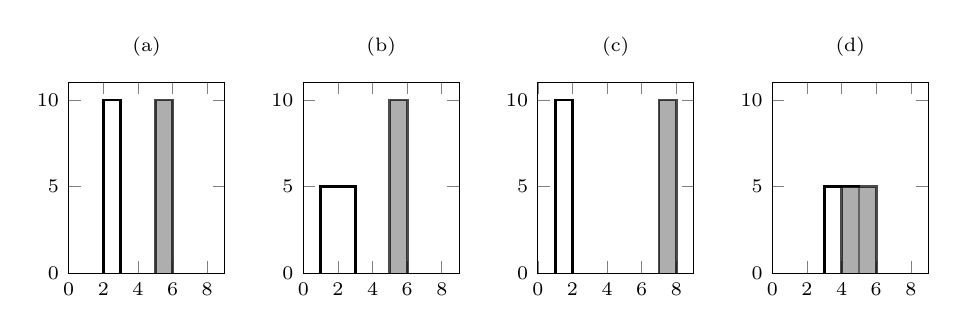
\begin{tikzpicture}
		
		% Chiều rộng thực tế (không đổi)
		\pgfmathsetmacro{\widthA}{0.1}
		\pgfmathsetmacro{\heightA}{1/\widthA}

		
		\pgfmathsetmacro{\widthBleft}{0.2}
		\pgfmathsetmacro{\heightBleft}{1/\widthBleft}
		\pgfmathsetmacro{\widthBright}{0.1}
		\pgfmathsetmacro{\heightBright}{1/\widthBright}
		
		\pgfmathsetmacro{\widthC}{0.2}
		\pgfmathsetmacro{\heightC}{1/\widthC}
		
		
		\begin{groupplot}[
			group style={group size=4 by 1, horizontal sep=1cm},
			width=4cm, height=4cm,
			axis equal image,
			axis lines=box,
			xmin=0, xmax=9, ymin=0, ymax=11,
			xtick={0,2,4,6,8},
			ytick={0,5,10},
			xticklabel style={font=\scriptsize},
			yticklabel style={font=\scriptsize}
			]
			
			% (a) same independent
			\nextgroupplot[title={\scriptsize (a)}]
			\addplot+[mark=none,draw=black,line width=1pt]
			coordinates {(2,0) (2,\heightA) (3,\heightA) (3,0)};
			\addplot+[mark=none,draw=black,line width=1pt,opacity=0.7, fill=black!45]
			coordinates {(5,0) (5,\heightA) (6,\heightA) (6,0)};
			
			
			% (b) uneven independent
			\nextgroupplot[title={\scriptsize(b)}]
			\addplot+[mark=none,draw=black,line width=1pt]
			coordinates {(1,0) (1,\heightBleft) (3,\heightBleft) (3,0)};
			\addplot+[mark=none,draw=black,line width=1pt,opacity=0.7, fill=black!45]
			coordinates {(5,0) (5,\heightBright) (6,\heightBright) (6,0)};
			
						% (d) p ⊂ q
			\nextgroupplot[title={\scriptsize(c)}]
			\addplot+[mark=none,draw=black,line width=1pt]
			coordinates {(1,0) (1,\heightA) (2,\heightA) (2,0)};
			\addplot+[mark=none,draw=black,line width=1pt,opacity=0.7, fill=black!45]
			coordinates {(7,0) (7,\heightA) (8,\heightA) (8,0)};
			
			
			% (c) overlapping
			\nextgroupplot[title={\scriptsize(d)}]
			\addplot+[mark=none,draw=black,line width=1pt]
			coordinates {(3,0) (3,\heightC) (5,\heightC) (5,0)};
			\addplot+[mark=none,draw=black,line width=1pt,opacity=0.7, fill=black!45]
			coordinates {(4,0) (4,\heightC) (6,\heightC) (6,0)};
			

			
		\end{groupplot}
		
	\end{tikzpicture}
	

	
\end{document}
